\section{Grundlagen}
\label{sec:Grundlagen}

In diesem Abschnitt werden die Grundlagen des Deep Learning und zweier häufig verwendeter Modelle erläutert.
Dies dient einer schrittweisen Heranführung an das letztendlich verwendete Modell.
Anschließend werden einige Beispiele für verwandte Forschung erläutert, um Ansätze herauszuarbeiten, die für die vorliegende Problemstellung eine geeignete Lösung sein könnten.

\subsection{Deep Learning}
\label{sec:DeepLearning}


\subsection{Long Short Term Memory}
\label{sec:LSTM}

Die einzige bisher vorgestellte Architektur von \acrshortpl{nn} ist das Feedforward-Netz.
Diese Netzarchitektur eignet sich gut für Klassifizierungsaufgaben.
Die vorliegende Arbeit beschäftigt sich jedoch mit Standorten von mobilen Radarkontrollen über die Zeit, also mit sequenziellen Daten.
Feedforward-Netze können zeitliche Zusammenhänge nicht darstellen und nicht erlernen, da sie keinen internen Zustand haben.
Das bedeutet, dass die Ausgabe des \acrshort{nn}s nur abhängig von der aktuellen Eingabe ist, nicht aber von vorherigen Eingaben.

Abhilfe hierbei bieten \k{rekurrente neuronale Netze} (\acrshortpl{rnn}).
Wie Chollet in \cite[S. 252]{DeepLearningPythonKeras} erläutert, besitzen rekurrente \acrshortpl{nn} einen internen Zustand, der alle bisherigen Eingaben repräsentiert.
Eine Ausgabe ist dann sowohl von der Eingabe als auch vom internen Zustand abhängig.
Implementiert wird dieses Verhalten durch eine Schleife im \acrshort{nn}.
In \autoref{fig:RNNSchleife} ist diese Architektur schematisch dargestellt.

\begin{figure}[h]
    \centering
    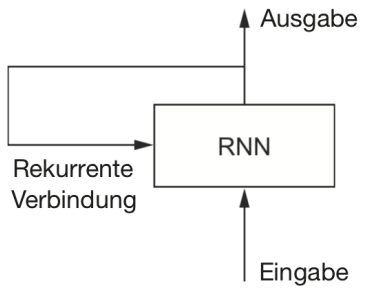
\includegraphics[width=0.5\textwidth,height=4cm,keepaspectratio=true]{content/images/RNNSchleife.png}
    \caption{Schleife in einem \acrshort{rnn} \cite[Abb. 6.9]{DeepLearningPythonKeras}}
    \label{fig:RNNSchleife}
\end{figure}

Ein einfaches \acrshort{rnn} berechnet die Ausgabe $Y_t$ nach \cite[S. 253]{DeepLearningPythonKeras} wie in \autoref{eq:RNN} gezeigt.

\begin{equation}
    Y_t = a(W \cdot X_t + U \cdot S_t + b)
\label{eq:RNN}
\end{equation}

Dabei steht $X_t$ für die Eingabe und $S_t$ für den internen Zustand, jeweils zum Zeitschritt $t$.
$W$ und $U$ sind Matrizen, die die trainierbaren Gewichtungen enthalten und $b$ ist ein trainierbarer Bias-Vektor.
Nach der Berechnung wird die Ausgabe zum neuen internen Zustand, man könnte also $S_t$ in \autoref{eq:RNN} durch $Y_{t-1}$ ersetzen.

Diese einfache Architektur unterliegt nach \cite[S. 260]{DeepLearningPythonKeras} jedoch dem sogenannten \emph{Problem des verschwindenden Gradienten}.
Dieser Effekt sorgt dafür, dass relativ weit zurückliegende Eingaben praktisch keinen Einfluss mehr auf die Ausgabe haben.
Es sind jedoch Anwendungsfälle denkbar, in denen auch weiter zurückliegende Ereignisse einen großen Einfluss auf die Gegenwart haben.
Für die Vorhersage von mobilen Radarkontrollen könnte beispielsweise von Bedeutung sein, wie die Verteilung der Radarkontrollen vor 15 Tagen ausgesehen hat.
Das liegt daran, dass die Daten eine Periodizität von z.B. 15 Tagen aufweisen könnten.

Zur Lösung dieses Problems gibt es verschiedene alternative \acrshort{rnn}-Architekturen.
Eine davon ist \acrfull{lstm}.
Wie der Name vermuten lässt, ermöglicht die \acrshort{lstm}-Architektur, sowohl Abhängigkeiten von weit zurückliegenden als auch aktuellere Eingaben zu lernen.
Die \acrshort{lstm}-Architektur ist in \autoref{fig:LSTMCell} dargestellt.

\begin{figure}[h]
    \centering
    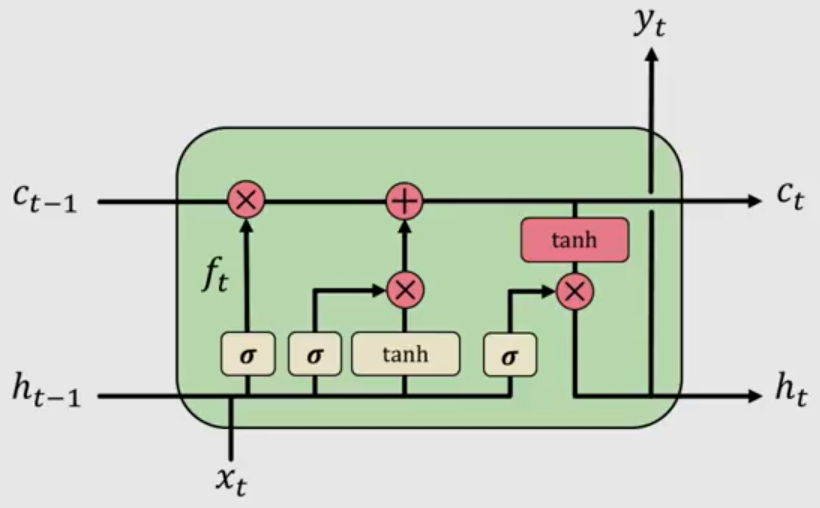
\includegraphics[width=0.8\textwidth,height=6cm,keepaspectratio=true]{content/images/LSTMCell.png}
    \caption{Schematische Darstellung einer \acrshort{lstm}-Zelle \cite{6S191RNN}}
    \label{fig:LSTMCell}
\end{figure}

Eine \acrshort{lstm}-Zelle enthält drei sogenannte Tore (engl. Gates).
Ein Tor ist selbst ein \acrshort{nn}.
Die drei Tore und ihre jeweilige vorgesehene Wirkung sind nach \cite{6S191RNN}:

\begin{enumerate}
    \setlength\itemsep{0.2em}
    \item \textbf{Vergessens-Tor}: Dieses Tor sorgt dafür, dass irrelevante Informationen aus dem vorherigen Zustand "`vergessen"' werden.
    \item \textbf{Merk-Tor}: Dieses Tor fügt dem Zustand relevante neue Informationen hinzu.
    \item \textbf{Ausgangs-Tor}: Dieses Tor bestimmt, welche Informationen aus dem Zustand zum Ausgang der Zelle gelangen sollen.
\end{enumerate}

Amini und Soleimany stellen die vorgesehene Wirkung der Tore in \cite{6S191RNN} ohne weitere kritische Auseinandersetzung dar.
Wie Chollet in \cite[S. 263]{DeepLearningPythonKeras} argumentiert, ist diese Wirkung jedoch keinesfalls garantiert.
Die tatsächliche Wirkung hinge nach Chollet viel mehr von den letzendlich antrainierten Gewichtungen der Tore ab.
Amini und Soleimany sind sich jedoch mit Chollet einig, dass es nicht wichtig ist, die interne Funktionsweise einer \acrshort{lstm}-Zelle im Detail zu verstehen.
Chollet geht noch einen Schritt weiter und argumentiert, dass dies ganz allgemein keine Aufgabe der Menschen sei.
Wichtig ist nach Chollet, Amini und Soleimany nur sich im klaren zu sein, welche Aufgabe eine \acrshort{lstm}-Zelle erfüllt - sie ermöglicht es, sowohl langfristige als auch kurzfristige Zusammenhänge anhand der Trainingsdaten zu erlernen.

\subsection{Faltungsnetze}
\label{sec:CNN}

Mit der bisher vorgestellten \acrshort{lstm}-Architektur können die zeitlichen Zusammenhänge bei der Vorhersage von mobilen Radarkontrollen erlernt werden.
Jedoch wurde bereits motiviert, warum auch räumliche Zusammenhänge für diese Aufgabenstellung von Bedeutung sind.
Prinzipiell ist es möglich, 2D-Daten mit Feedforward-Netzen zu verarbeiten.
Dazu müssen die 2D-Daten verflacht werden.
Für ein zweidimensionales Bild bedeutet das, dass jedes Pixel einem Eingangsneuron zugeführt wird.
Hierbei geht die räumliche Struktur der Daten jedoch verloren.
Das \acrshort{nn} kann nicht wissen, welche Pixel in alle vier Richtungen benachbart waren.
Mit genug Trainingsdaten können einfache Klassifizierungsaufgaben dennoch mit dieser Netzarchitektur bearbeitet werden.
Chollet demonstriert beispielsweise in \cite[S. 53]{DeepLearningPythonKeras}, dass bei der Klassifizierung von handgeschriebenen Ziffern mit einem Feedforward-Netz eine Korrektklassifizierungsrate von 97,8\,\% erreicht werden kann.
Das Problem mit Feedforward-Netzen ist jedoch, dass sie nur globale Muster erlernen, also beispielsweise eine Ziffer als Ganzes.
Ist dieselbe Ziffer nun etwas im Bild verschoben oder auf sonstige Weise verzerrt, wird sie von einem Feedforward-Netz nicht mehr erkannt.
Dies kann dadurch visualisiert werden, dass nach einer Verzerrung die einzelnen Pixel an ganz anderen Eingangsneuronen anliegen.

Abhilfe hierbei verschaffen Faltungsnetze (engl. \acrlongpl{cnn}, \acrshortpl{cnn}).
\acrshortpl{cnn} entsprechen dem Stand der Technik, wenn es um die Verarbeitung von 2D-Daten geht.
Wenn das vorherige Beispiel nochmals betrachtet wird, kann man erkennen, welche Eigenschaften der Ziffern sich nicht durch eine Verzerrung ändern: Die Zusammensetzung der Ziffern aus kleineren Merkmalen.
Selbst wenn eine Ziffer verschoben oder leicht verzerrt wird, werden sich (relativ zueinander) immer noch dieselben Linien an denselben Stellen kreuzen oder berühren.
Die Betrachtung von 2D-Daten als Zusammensetzung von lokalen Mustern wird in \autoref{fig:LokaleMuster} verdeutlicht.

\begin{figure}[h]
    \centering
    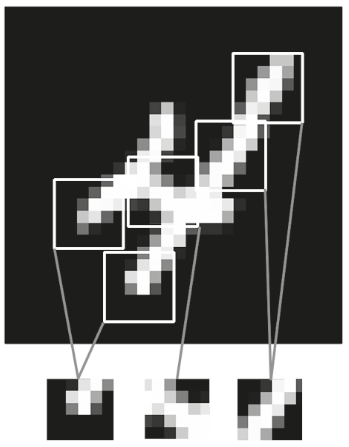
\includegraphics[width=0.4\textwidth,height=4cm,keepaspectratio=true]{content/images/LokaleMuster.png}
    \caption{Lokale Muster wie Ränder und Linien in einer handgeschriebenen Ziffer \cite[Abb. 5.1]{DeepLearningPythonKeras}}
    \label{fig:LokaleMuster}
\end{figure}

\acrshortpl{cnn} erkennen nach \cite[S. 164]{DeepLearningPythonKeras} nun diese lokalen Muster.
Chollet geht in \cite{DeepLearningPythonKeras} auf Seite 165 auf die daraus resultierenden Eigenschaften von \acrshortpl{cnn} ein.
Zunächst sei die Erkennung der lokalen Muster translationsinvariant.
Dies bedeute, dass die Muster an beliebigen Stellen im Bild erkannt werden können.
Außerdem könne durch das Hintereinanderschalten mehrer \acrshort{cnn}-Layer erreicht werden, dass Hierarchien von Mustern erlernt werden.
Aus diesen beiden Eigenschaften folgt, dass es für ein \acrshort{cnn} keinen Unterschied macht, ob die zu erkennenden globalen Muster (beispielsweise eine Ziffer) in der Eingabe verschoben sind.

Als Nächstes stellt sich die Frage, wie \acrshortpl{cnn} lokale Muster erkennen können.
Dies wird durch die Faltungsoperation erreicht.
Die Idee der Faltungsoperation ist nach \cite{6S191CNN}, einen sogenannten Filter zu verwenden, der lokale Muster erkennt.
Dieser zweidimensionale Filter wird über die 2D-Eingabe "`geschoben"' und erkennt somit, wo sich in der Eingabe ein bestimmtes Muster befindet.
Mathematisch gesehen ist ein Filter eine quadratische Matrix.
Die Elemente der Matrix sind die erlernbaren Gewichtungen, die je nach ihren Werten verschiedene Muster erkennen.
Die Erkennung geschieht dadurch, dass der Filter an der jeweiligen Stelle komponentenweise mit der Eingabe multipliziert und die einzelnen Werte anschließend aufsummiert werden.
Diese Berechnung wird in \autoref{fig:ConvExample} verdeutlicht.

\begin{figure}[h]
    \centering
    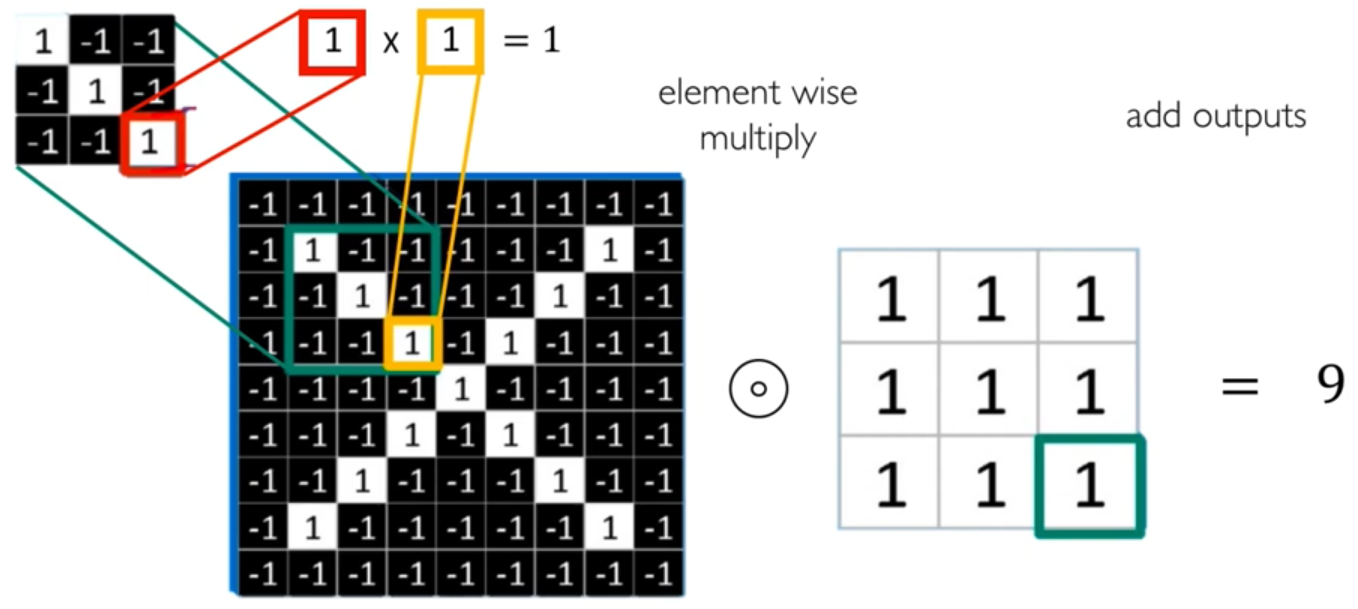
\includegraphics[width=1.0\textwidth,height=8cm,keepaspectratio=true]{content/images/ConvExample.png}
    \caption{Ein Schritt der Faltung des Filters mit der Eingabe \cite{6S191CNN}}
    \label{fig:ConvExample}
\end{figure}

Links oben in der Abbildung ist der Filter dargestellt.
Dieser Filter erkennt schräge Linien von links oben nach rechts unten.
Bei einer perfekten Übereinstimmung, wie im Beispiel der Abbildung, wird das Ergebnis der Berechnung maximal.
Angenommen, das Pixel oben in der Mitte der Eingabe wäre $1$, dann wäre das Ergebnis der Berechnung nur $7$.
Der Wert des Ergebnisses ist also ein Maß für die Übereinstimmung des Filters mit der Eingabe.
Auf dieses Ergebnis wird in der Praxis nach \cite{6S191CNN} noch eine Aktivierungsfunktion angewendet, wofür meistens \emph{\acrshort{relu}} verwendet wird.
Negative Pixel werden dadurch zu null.
Wird der Filter nun mit einer Schrittweite von $1$ in $x$- und $y$-Richtung über die gesamte Eingabe geschoben und die Berechnung jedes Mal ausgeführt, entsteht eine sogenannte Merkmalskarte (engl. \emph{feature map}).
Die Merkmalskarte gibt an, wo im Bild die Übereinstimmung mit dem durch den Filter beschriebenen Muster wie groß ist.
Damit die Merkmalskarte die gleiche Höhe und Breite wie die Eingabe hat, kann nach \cite[S. 168 f.]{DeepLearningPythonKeras} die Eingabe vor der Faltungsoperation rundherum mit Nullen aufgefüllt werden.
Dies wird auch \emph{Padding} genannt.

Nach der Faltungsoperation ist noch ein weiterer wichtiger Schritt notwendig.
Da die Merkmalskarte zunächst die gleichen Dimensionen wie die Eingabe hat, können nach \cite[S. 171]{DeepLearningPythonKeras} keine Merkmalshierarchien erkannt werden.
Das liegt daran, dass ein Pixel der Merkmalskarte nur Informationen über einen Bereich der Eingabe enthält, der so groß ist wie der Filter.
In den meisten Fällen sind dies nur 3x3 oder 5x5 Pixel.
Das Ziel ist es also, eine Merkmalskarte zu erstellen, bei der ein Pixel Informationen über einen größeren Bereich der Eingabe enthält.
Dies kann durch die MaxPooling-Operation erreicht werden, die auf die Merkmalskarte angewendet wird.
Diese funktioniert ähnlich wie die Faltungsoperation.
Auch hier gibt es einen Filter, der über die Eingabe geschoben wird.
Dieser Filter wird hier jedoch als \emph{Pool} bezeichnet.
Im Gegensatz zur Faltungsoperation wird nichts multipliziert.
Stattdessen entspricht die Ausgabe des Pools dem Maximalwert der Eingabe.
Hat der Pool beispielsweise eine Größe von 2x2 und wird in $x$- und $y$-Richtung jeweils um die Schrittweite $2$ verschoben, wird die Seitenlänge der Eingabe durch die MaxPooling-Operation halbiert.
Dies wird in \autoref{fig:MaxPooling} an einem Beispiel veranschaulicht.

\begin{figure}[h]
    \centering
    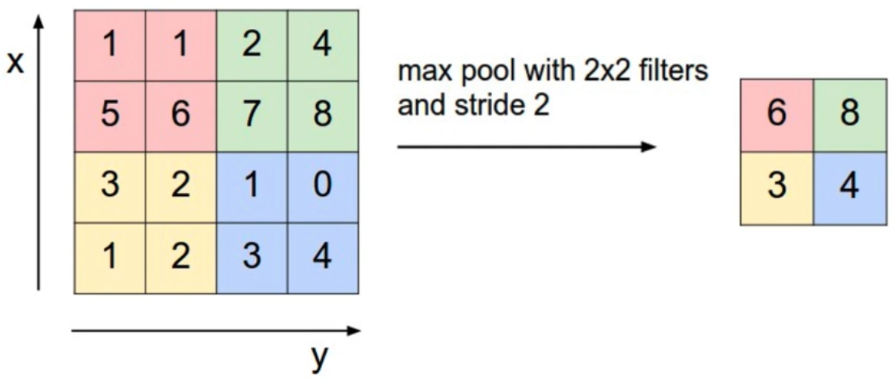
\includegraphics[width=0.8\textwidth,height=8cm,keepaspectratio=true]{content/images/MaxPooling.png}
    \caption{Beispiel einer MaxPooling-Operation \cite{6S191CNN}}
    \label{fig:MaxPooling}
\end{figure}

Werden mehrere \acrshort{cnn}- und MaxPooling-Layer abwechselnd hintereinandergeschaltet, lassen sich die Merkmale der Eingabe hierarchisch darstellen.
Dabei wird die Höhe und Breite der Eingabe nach jedem MaxPooling-Layer halbiert.
Zumm Schluss wird die Ausgabe des letzten MaxPooling-Layers an ein Feedforward-Netz zur Klassifizierung übergeben.
Das Feedforward-Netz klassifiziert die Eingabe also nun anhand von abstrakten Merkmalen, die durch die \acrshort{cnn}- und MaxPooling-Layer von \emph{beliebigen Stellen} in der Eingabe extrahiert wurden.

\subsection{TensorFlow}
\label{sec:TensorFlow}

TensorFlow ist eine Python-Bibliothek für viele verschiedene Machine Learning Aufgaben.
TensorFlow implementiert dafür u.A. mathematische Grundfunktionen wie Tensoroperationen oder die Gradientenberechnung.
Da sehr viel Fachwissen nötig wäre um alleine mit TensorFlow \acrshortpl{nn} zu implementieren, wird mit TensorFlow auch die Keras-Bibliothek ausgeliefert.
Keras baut auf TensorFlow auf und bietet ein High-Level-Framework für neuronale Netze.
Mit Keras können \acrshortpl{nn} relativ einfach definiert, trainiert und ausgewertet werden.
Keras bietet sehr viele vordefinierte Layer, darunter Feedforward-, \acrshort{lstm}-, \acrshort{cnn}- sowie MaxPooling-Layer.
Bei Bedarf können jedoch auch auch eigene Layer definiert werden.
Aus diesen vordefinierten und ggf. benutzerdefinierten Layern können beliebig komplexe Modelle zusammengesetzt werden.
Außerdem kann der Ablauf des Trainings dieser Modelle komplett angepasst werden, inklusive des Optimierers und der Verlustfunktion.
Da die Trainierung von \acrshortpl{nn} sehr rechenintensiv ist, bietet TensorFlow die Möglichkeit, die Berechnungen auf einer Grafikkarte auszuführen.
Da Grafikkarten Berechnungen hochgradig parallelisiert ausführen, können Modelle deutlich schneller trainiert werden als auf der CPU.

\subsection{Formale Problemdefinition räumlich-zeitlicher Vorhersagen}
\label{sec:STPredictions}
Im Themenfeld der räumlich-zeitlichen Vorhersagen (engl. \emph{spatio-temporal predictions}) gibt es viele verschiedene Anwendungsfälle.
Zu diesen Anwendungsfällen gehört die Vorhersage von Niederschlägen, Verbrechen, Verkehrsunfällen, Verkehrsaufkommen sowie der Bedarf an Taxis \cite{ConvLSTM,CrimeConvLSTM,CrimeSTResNet,HeteroConvLSTM,TrafficVolumeGraphDCRNN,STResNetOriginal}.
So unterschiedlich die Themengebiete auch sind, lässt sich laut \cite{DLTraff} dennoch eine gemeinsame, formale Problemstellung definieren.
Wenn die Daten als Raster vorliegen, können sie als 4D-Tensor $\mathbb{R}^{T \times H \times W \times C}$ beschrieben werden.
Dabei ist $T$ die Anzahl der Zeitschritte, $H \times W$ die räumliche Dimension (Höhe mal Breite) und $C$ die Anzahl an Kanälen.
Besteht der Datensatz beispielsweise aus 100 \acrshort{rgb}-Bildern mit einer Größe von 28x28 Pixel, kann er mit dem Tensor $\mathbb{R}^{100 \times 28 \times 28 \times 3}$ beschrieben werden.
Die Problemstellung lässt sich nun als die in \autoref{eq:FormalSTPrediction} gezeigte Abbildung $f$ formulieren.

\begin{equation}
    f: [X_{t-(\alpha-1)}, \dots, X_{t-1}, X_t] \to [X_{t+1}, X_{t+2}, \dots, X_{t+\beta}]
\label{eq:FormalSTPrediction}
\end{equation}

Dabei repräsentiert $X_t \in \mathbb{R}^{H \times W \times C}$ ein Raster zum Zeitpunkt $t$.
Außerdem ist $\alpha$ die Anzahl an Zeitschritten, anhand derer die Vorhersage getroffen wird und $\beta$ die Anzahl an Zeitschritten, die vorhergesagt werden soll.
Es ist auch möglich, nur einen Zeitschritt vorherzusagen.
Wenn beispielsweise anhand von 16 vergangenen Tagen der 17. Tag vorhergesagt werden soll, dann ist $\alpha = 16$ und $\beta = 1$.
Daraus ergibt sich $g: [X_{t-15}, X_{t-14}, \dots, X_{t-1}, X_t] \to X_{t+1}$.
Mit $g$ ist nun die Funktion definiert, die in der vorliegenden Arbeit durch ein \acrshort{nn} approximiert werden soll.

Obwohl eine solche allgemeine Definition der Problemstellung möglich ist, gibt es dennoch große Unterschiede, wenn die Definition auf verschiedene Datensätze angewendet wird.
Das liegt vor allem daran, dass die Datensätze eine sehr unterschiedliche Sturkur haben und sehr unterschiedlichen Gesetzmäßigkeiten unterliegen.
Zunächst gibt es Unterschiede in der räumlichen Struktur der Daten.
Grundsätzlich können die Daten räumlich diskret oder kontinuierlich sein.
Ein Beispiel für räumlich diskrete Daten sind Wetterdaten.
Diese werden von Wetterstationen an bestimmten Orten aufgenommen, die sich über die Zeit nicht ändern.
Beispiele für räumlich kontinuierliche Daten sind Verkehrsunfälle oder Verbrechen.
Diese können an beliebigen Orten bzw. Koordinaten auftreten.
Räumlich kontinuierliche und diskrete Daten können in beide Richtungen umgewandelt werden.
Räumlich diskrete Daten können in räumlich kontinuierliche Daten umgewandelt werden, indem zweidimensional interpoliert wird.
Hingegen können räumlich kontinuierliche Daten in räumlich diskrete Daten umgewandelt werden, indem Cluster bzw. Hotspots in den Daten identifiziert werden.
Alle Datenpunkte, die zu einem Cluster gehören, bekommen dann als Koordinaten den Schwerpunkt des Clusters zugeordnet.
Die Voraussetzung für dieses Vorgehen ist jedoch, dass überhaupt Cluster in den Daten erkennbar sind.

Unabhängig davon, ob die Daten ursprünglich räumlich diskret oder kontinuierlich vorliegen, lassen sie sich grundsätzlich auf zwei verschiedene Arten repräsentieren: als Raster oder als Graph.
Sollen die Daten als Raster repräsentiert werden, wird ein zunächst leeres Raster aus gleichgroßen, meist quadratischen Zellen über die Daten gelegt.
Anschließend werden jeder Rasterzelle diejenigen Datenpunkte zugeordnet, die innerhalb der Zelle liegen.
Da jede Rasterzelle aus nur einem Zahlenwert besteht, muss eine bestimmte Metrik festgelegt werden, anhand derer dieser Zahlenwert bestimmt wird.
Dies könnte beispielsweise die Anzahl der Datenpunkte innerhalb eines bestimmten Zeitraums sein.
Alternativ könnte eine bestimmte Eigenschaft der Datenpunkte aufsummiert werden.
Sollen die Daten hingegen als Graph repräsentiert werden, müssen sie zunächst räumlich diskret vorliegen.
Liegen die Daten räumlich kontinuierlich vor, müssen zuerst Cluster gebildet werden.
Jeder diskrete Ort bzw. jedes Cluster wird dann ein Knoten des Graphs.
Anschließend muss festgelegt werden, welche Verbindungen zwischen den einzelnen Knoten bestehen.
Hier bietet es sich an, Verbindungen festzulegen, die in der Realität auch bestehen.
Dies könnte beispielsweise das Straßennetz sein, wenn es sich um Verkehrsdaten handelt.

Nicht nur in der räumlichen Struktur der Daten kann es Unterschiede geben, sondern auch in der zeitlichen Struktur.
So lassen sich Datensätze im Bezug auf die zeitliche Struktur in zwei Kategorien einteilen: Die Datenpunkte können entweder in regelmäßigen oder in unregelmäßigen Zeitabständen vorliegen.
Wetterstationen liefern beispielsweise Messwerte in regelmäßigen Zeitabständen.
Verkehrsunfälle geschehen hingegen in unregelmäßigen Zeitabständen.
Eine weitere Eigenschaft der Daten ist die zeitliche Auflösung, also der (durchschnittliche) Zeitabstand einzelner Datenpunkte.
Wetterstationen liefern beispielsweise Daten in sehr kurzen Zeitabständen.
Daher können schon in einem relativ kurzen Zeitraum sehr viele Daten gesammelt werden.
Verkehrsunfälle oder Verbrechen treten im Gegensatz dazu nur sehr sporadisch auf.
Daher müssen Daten über einen sehr langen Zeitraum gesammelt werden, um auf deren Basis Vorhersagen treffen zu können.
Insgesamt ist zeitliche Auflösung wichtig, da sie die erzielbare Genauigkeit und die zeitliche Auflösung der Vorhersagen beschränkt.

Die verschiedenen Möglichkeiten der Kombination von räumlicher und zeitlicher Beschaffenheit der Daten ist mit Beispielen in \autoref{tab:STStructureUseCases} zusammengefasst.

\begin{table}[h]
\centering
\begin{tabular}{|l|l|l|}
\hline
 & \textbf{Räumlich kontinuierlich} & \textbf{Räumlich diskret} \\ \hline
\textbf{\begin{tabular}[c]{@{}l@{}}Regelmäßige\\ Zeitabstände\end{tabular}} & \begin{tabular}[c]{@{}l@{}}Regelmäßig gesendete\\ GPS-Daten\end{tabular} & Wetterstationen \\ \hline
\textbf{\begin{tabular}[c]{@{}l@{}}Unregelmäßige\\ Zeitabstände\end{tabular}} & \begin{tabular}[c]{@{}l@{}}Verkehrsunfälle, Verbrechen,\\ mobile Radarkontrollen\end{tabular} &  \\ \hline
\end{tabular}
\caption{Beispiele für Anwendungsfälle mit verschiedenen räumlichen und zeitlichen Strukturen der Daten}
\label{tab:STStructureUseCases}
\end{table}

Zuletzt gibt es noch den Unterschied zwischen kontinuierlich gemeldeten Messwerten und sporadisch auftretenden Ereignissen.
Während der Zahlenwert einer Messung zu einem bestimmten Zeitpunkt intuitiv klar ist, ist dies bei Ereignissen nicht sofort klar.
Für die Behandlung von Ereignissen gibt es mehrere Möglichkeiten.
Zum einen kann ein Ereignis als ein Messwert mit dem immer gleichen Zahlenwert "`$1$"' betrachtet werden.
Zum anderen kann dem Ereignis ein Zahlenwert zugeordnet werden, der das Ereignis bzw. dessen Signifikanz genauer beschreibt.
Für mobile Radarkontrollen könnte dieser Zahlenwert beispielsweise die Standdauer sein.

\subsection{Neuronale Netze für räumlich-zeitliche Vorhersagen}
\label{sec:STNNs}

Um räumlich-zeitliche Zusammenhänge in Datensätzen durch ein \acrshort{nn} zu erlernen existieren verschiedene Architekturen.
In \cite{DLTraff} befindet sich ein detaillierter Vergleich vieler dieser Architekturen anhand ihrer Ansätze und Performance.
Zwei weit verbreitete Beispiele werden im folgenden zusammengefasst.

\textbf{ST-ResNet} wird in \cite{STResNetOriginal} definiert und ist eines der populärsten Modelle für räumlich-zeitliche Vorhersagen.
In \cite{DLTraff} wird dies mit der großen Anzahl an Paper begründet, die Referenzen auf \cite{STResNetOriginal} enthalten.
Der Anwendungsfall für den ST-ResNet konzipiert wurde, ist die Vorhersage der Bewegung von Menschenmassen (engl. \emph{crowd flow}).
Dabei ist es egal, wie sich die Menschen bewegen.
So kann ST-ResNet beispielsweise nicht nur auf Fußgänger angewendet werden, sondern auch auf Leihfahrräder, Taxis oder Verkehr allgemein.
Außerdem kann ST-ResNet auch auf beliebige andere rasterbasierte räumlich-zeitliche Vorhersagen angewendet werden, wie z. B. die Vorhersage von Verbrechen.
Diese konkrete Adaption wird von den Autoren von ST-ResNet in \cite{CrimeSTResNet} gezeigt.
Ein Datensatz, für den ST-ResNet ursprünglich konzipiert wurde, besteht aus einem Raster über viele Zeitschritte.
Pro Zeitschritt sind jeder Zelle zwei Werte zugeordnet: die Anzahl an Menschen, die die Zelle betreten (engl. \emph{inflow}) und die Anzahl an Menschen, die die Zelle verlassen (engl. \emph{outflow}).
Dies ist ein Beispiel für einen Datensatz mit zwei Kanälen.
Für die Architektur von ST-ResNet haben sich Zhang et al. genau überlegt, welche räumlichen und zeitlichen Zusammenhänge in den Daten vorhanden sein könnten.
Sie stellen zunächst fest, dass der Inflow einer Zelle abhängig ist vom Outflow der benachbarten Zellen.
Es können jedoch auch Zusammenhänge zu weiter entfernten Zellen bestehen, da es in größeren Städten normalerweise ein U-Bahn Netz gibt, welches weiter entfernte Zellen direkt miteinander verbindet.
Bei den zeitlichen Zusammenhängen handelt es sich um verschieden große Zeitspannen.
Zhang et al. führen je Beispiele für Zusammenhänge innerhalb eines Tages sowie für tagliche, wöchentliche und jährliche Zusammenhänge an.
Beispielsweise würden sich die Bewegungen von Menschenmassen zu Stoßzeiten jeden Tag ähnlich verhalten, wobei die Stoßzeiten im Winter aufgrund des späteren Sonnenaufgangs ebenfalls später auftreten würden.
Die Bewegungen im Allgemeinen würden zusätzlich zu den räumlichen und zeitlichen Begebenheiten auch von externen Faktoren wie dem Wetter beeinflusst.
Um alle diese möglichen Zusammenhänge zu berücksichtigen, haben Zhang et al. die in \autoref{fig:STResNetArchitecture} dargestellte Architektur entworfen.

\begin{figure}[h]
    \centering
    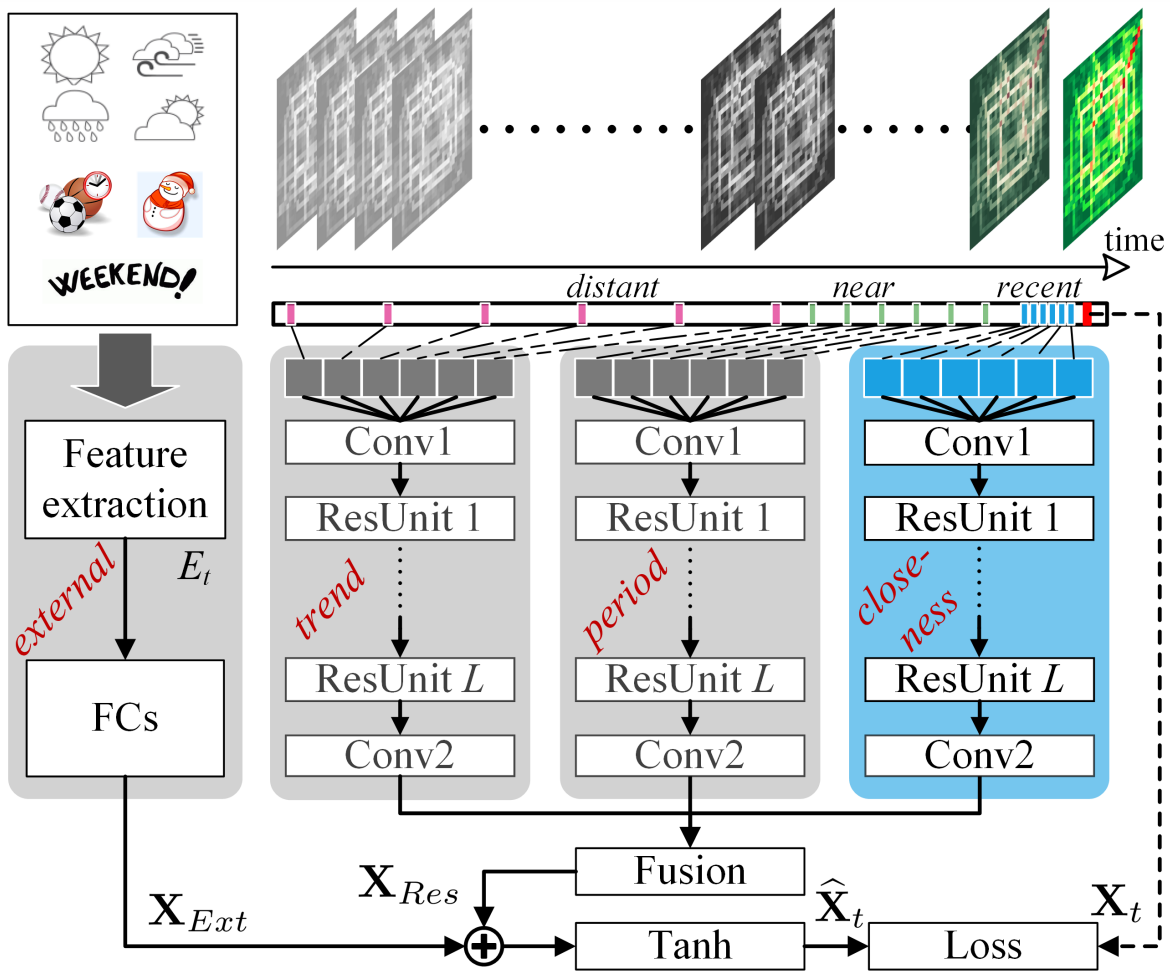
\includegraphics[width=0.8\textwidth,height=10cm,keepaspectratio=true]{content/images/STResNetArchitecture.png}
    \caption{Architektur von ST-ResNet \cite[Figure 3]{STResNetOriginal}}
    \label{fig:STResNetArchitecture}
\end{figure}

ST-ResNet besteht im Wesentlichen aus vier Teilen, die in \autoref{fig:STResNetArchitecture} eingerahmt sind.
Die drei rechten Teile modellieren den langfristigen Trend (\emph{trend}), mittelfristige Periodizitäten (\emph{period}) und kurzfristige Begebenheiten (\emph{closeness}).
Diese drei Teile haben jeweils die gleiche Struktur.
Die Eingangsdaten werden zunächst einem \acrshort{cnn}-Layer zugeführt.
Dessen Ausgabe durchläuft dann mehrere sogenannte Residual Units.
Diese beinhalten wiederum \acrshort{cnn}-Layer, jedoch wird die Eingabe einer Residual Unit wieder zum Ausgang der \acrshort{cnn}-Layer dazuaddiert.
Dadurch können sehr tiefe Netze gebildet werden, ohne dass diese dem Problem des verschwindenden Gradienten unterliegen.
Der Ausgang der letzten Residual Unit wird schlussendlich nochmals durch einen \acrshort{cnn}-Layer verarbeitet.

Der Unterschied dieser drei rechten Teile liegt in den Eingangsdaten.
Der \emph{trend}-Teil erhält als Eingangsdaten Zeitschritte im Abstand von einer Woche, die über die gesamte Zeitspanne des Datensatzes verteilt sind.
Somit kann die langfristige Entwicklung der Daten erlernt werden, wie auch wöchentliche Periodizitäten.
Der \emph{period}-Teil erhält Zeitschritte im Abstand von einem Tag, die nicht sehr lange zurückliegen.
Damit können tägliche Periodizitäten erlernt werden, wie die bereits erwähnten Stoßzeiten.
Zuletzt erhält der \emph{closeness}-Teil alle verfügbaren Zeitschritte der letzten paar Tage.
Anhand dessen kann die momentane Situation erkannt werden.
Diese Ausgaben dieser drei Teile werden schlussendlich gewichtet zusammengeführt.
Der in \autoref{fig:STResNetArchitecture} ganz links dargestellte Teil verarbeitet externe Daten durch ein vollständig verbundenes Netz.
Signifikante Merkmale, die als Eingabe dienen sollen, müssen hierfür manuell ermittelt werden.
Die Kombination aus dem linken Teil und der zusammengeführten Ausgabe der drei rechten Teile bildet schließlich die Ausgabe von ST-ResNet.

\textbf{ConvLSTM} ist ebenfalls eine weit verbreitete Architektur für räumlich-zeitliche Vorhersagen.
Conv\-LSTM wurde von Shi et al. in \cite{ConvLSTM} vorgestellt.
Bei ConvLSTM handelt es sich um eine Kombination aus \acrshort{cnn} und \acrshort{lstm}.
Durch Faltungsoperationen soll hierbei die räumliche Strukur erhalten bleiben.
Außerdem soll durch die Verwendung einer abgewandelten \acrshort{lstm}-Struktur die zeitlichen Zusammenhänge erfasst werden.
Das ursprüngliche Ziel von ConvLSTM ist nach Shi et al. die Vorhersage einer \emph{Sequenz} von 2D-Daten anhand einer Eingabesequenz.
Dafür orientieren sie sich an der in \cite{SequenceGeneratingLSTM} vorgestellten Architektur.
Diese Architektur besteht aus mehreren hintereinandergeschalteten \acrshort{lstm}-Zellen.
Jedoch wurde sie für die Generierung von 1D-Sequenzen konzipiert und verwendet daher Matrixmultiplikationen mit Gewichtungsmatrizen.
Diese werden von Shi et al. durch Faltungsoperationen ersetzt, wodurch zweidimensionale Strukturen erlernt werden können.
Diese Architektur wird in \autoref{fig:ConvLSTMStructure} verdeutlicht.

\begin{figure}[h]
    \centering
    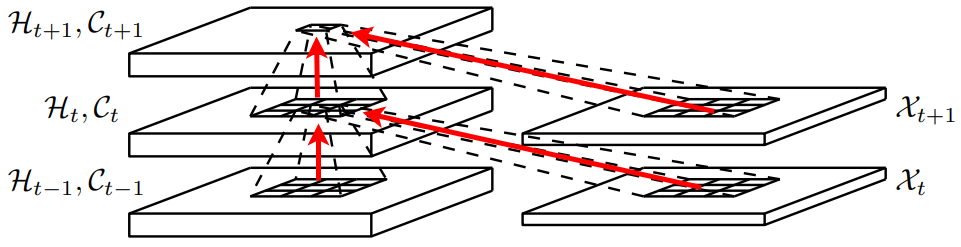
\includegraphics[width=0.8\textwidth,height=10cm,keepaspectratio=true]{content/images/ConvLSTMStructure.png}
    \caption{Innere Struktur von ConvLSTM aus \cite{ConvLSTM} mit hinzugefügten Pfeilen zur Verdeutlichung des Informationsflusses}
    \label{fig:ConvLSTMStructure}
\end{figure}

Wie man in der Abbildung erkennen kann, hängt jedes Pixel der Ausgabe von einem Bereich der Eingabe und einem Bereich des inneren Zustands ab.
Dadurch, dass die Tore aus der \acrshort{lstm}-Architektur übernommen wurden, werden von ConvLSTM auch die räumlich-zeitlichen Zusammenhänge nach ihrer Relevanz gefiltert.
Wie auch schon bei reinen \acrshortpl{lstm} ist es nicht wichtig zu verstehen, was genau die Tore räumlich und zeitlich filtern.
Es ist nur wichtig zu wissen, dass mit ConvLSTM lang- und kurzfristige Abhängigkeiten in der räumlichen und zeitlichen Dimension erlernt werden können.

% TODO: Evtl. Verschieben in ModellEntwurf
Prinzipiell sind beide Modelle für den Anwendungsfall der Vorhersage von mobilen Radarkontrollen geeignet, da beide Rasterbasiert arbeiten und räumliche sowie zeitliche Zusammenhänge erlernen können.
Für die Auswahl eines der Modelle kommen also vor allem praktische Aspekte in Betracht.
Dafür ist zunächst wichtig, dass die vorliegende Arbeit in einer begrenzten Zeit fertiggestellt werden muss.
Daher sollte es so wenig wie möglich Aufwand machen, das Modell in einer Implementierung zu verwenden.
Hier hat ConvLSTM den großen Vorteil, dass es bereits eine fertige Implementierung als Teil von TensorFlow bzw. Keras gibt: \emph{tf.keras.layers.ConvLSTM2D}\footnote{\url{https://www.tensorflow.org/api_docs/python/tf/keras/layers/ConvLSTM2D}}.
Im Gegensatz dazu gibt es für ST-ResNet keine Standardimplementierung, die ohne weiteres Verwendet werden kann.
Es existieren zwar unabhängige, auf TensorFlow basierende Implementierungen auf GitHub\footnote{\url{https://github.com/deepkashiwa20/DL-Traff-Grid/blob/master/workTaxiNYC/predflowio/ST_ResNet.py}}\textsuperscript{,}\footnote{\url{https://github.com/snehasinghania/STResNet}}, jedoch sind diese speziell auf den in \cite{STResNetOriginal} beschriebenden Anwendungsfall angepasst.
Daher müsste einiges an Zeit investiert werden, um die Implementierung zu verstehen und sie entsprechend an den vorliegenden Anwendungsfall anzupassen.
Mit der verfügbaren Implementierung von ConvLSTM als Teil von TensorFlow geht auch einher, dass einige Ressourcen existieren, die beschreiben, wie ConvLSTM praktisch angewendet werden kann.
Ein Beispiel hierfür ist das später noch verwendete Paper \cite{CrimeConvLSTM}.
Aufgrund dieser praktischen Vorteile wird in der vorliegenden Arbeit mit ConvLSTM weitergearbeitet.




% Verwandte Anwendungsfälle:
%   - Niederschlagsvorhersage als weiter entfernt
%   - Verbrechensvorhersage als sehr ähnlichen Anwendungsfall

\subsection{Verwandte Anwendungsfälle}
\label{sec:VerwandteAnwendungsfaelle}
In \autoref{sec:STPredictions} wurden bereits einige Anwendungsfälle von räumlich-zeitlichen Vorhersagen genannt.
In diesem Abschnitt sollen diese Anwendungsfälle im Bezug auf ihre Relevanz für die Vorhersage von mobilen Radarkontrollen genauer untersucht werden.

Anhand von \autoref{tab:STStructureUseCases} können die verschiedenen Anwendungsfälle schon grob in Kathegorien eingeteilt werden.
An der Tabelle ist außerdem zu erkennen, dass vor allem die Vorhersage von Verkehrsunfällen und Verbrechen eine große Relevanz für die vorliegende Problemstellung hat, da es sich dort ebenfalls um räumlich kontinuierliche Ereignisse handelt, die in unregelmäßigen Zeitabständen auftreten.
Eine weitere Eigenschaft dieser Anwendungsfälle ist, dass die Ereignisse nur sehr sporadisch auftreten.
Während Wetterstationen beispielsweise alle paar Sekunden einen Messwert liefern, treten pro Tag vergleichsweise wenige Verkehrsunfälle und Verbrechen pro Tag auf.
Bei mobilen Radarkontrollen verhält es sich ähnlich.
Beispielsweise werden in einem 50x50 km Bereich um Stuttgart herum im Durchschnitt pro Tag xxxTODOxxx mobile Radarkontrollen gemeldet.





%   - Niederschlagsvorhersage als weiter entfernt
%   - Verbrechensvorhersage als sehr ähnlichen Anwendungsfall

